%        File: DesignDocument.tex
%     Created: 一 3月 26 01:00 下午 2018 C
% Last Change: 一 3月 26 01:00 下午 2018 C
%
\documentclass[UTF8,noindent]{ctexart}
\usepackage[a4paper,left=2.0cm,right=2.0cm,top=2.0cm,bottom=2.0cm]{geometry}
\usepackage{hyperref}
\usepackage{url}
\usepackage{graphicx}
\usepackage{amsmath}
\usepackage{amssymb}
\usepackage{enumitem}
\usepackage{tikz}
\usepackage{float}
\usepackage{xeCJK}
\usepackage{listings}
\usepackage{xcolor}
\lstset{language = c,numbers=left, showstringspaces=false,keywordstyle= \color{ blue!70 },commentstyle=\color{red!50!green!50!blue!50}, frame=shadowbox, rulesepcolor= \color{ red!20!green!20!blue!20 } 
} 
\CTEXsetup[format={\Large\bfseries}]{section}
\usetikzlibrary{graphs}
%\newtheorem*{lemma}{Lemma}
\title{\CJKfamily{zhkai}计算机网络研讨课实验报告}
\author{{\CJKfamily{zhkai}冯吕}\ $2015K8009929049$}
\date{\today}
\begin{document}
\maketitle
\zihao{5}
\CJKfamily{zhsong}
%\begin{center}
%  \begin{tabular}{|p{15cm}|}
%    \hline
\section*{{\CJKfamily{zhhei}实验题目}}交换机学习实验 
%\hline
\section*{{\CJKfamily{zhhei}实验内容}}
在本次实验中,需要实现交换机的转发。在广播网络中,转发节点将每个数
据包从所有其他端口广播出去,而在交换网络中,交换机将收到的数据包沿着目的主机方向转发。

实现交换机的关键思想是:
\begin{quote}
  当交换机从某端口收到源$mac$地址为$X$的数据包时,那么,将数据包从该端口转出一定可以到达目的$mac$地址为$X$的目的主机。
\end{quote}

交换机需要实现如下操作:
\begin{itemize}
  \item 查询操作:每收到一个数据包,根据目的MAC地址查询相应转发条目:如果查
询到对应条目,则根据相应转发端口转发数据包,并更新访问时间;否则,广播该
数据包。
\item 插入操作:每收到一个数据包,如果其源MAC地址不在转发表中,则将该地址
与入端口的映射关系写入转发表。
\item 老化操作:每秒钟运行一次老化操作,删除超过30秒未访问的转发条目。
\end{itemize}

另外,转发表的老化操作与其他操作独立运行:通过多线程和互斥操作实现。\\

实验具体需要实现的内容是:数据结构$mac\_port\_map$的所有操作,以及数据包的转发和广播操作,对应的函数如下:
\begin{lstlisting}
iface_info_t *lookup_port(u8 mac[ETH_ALEN]);

void insert_mac_port(u8 mac[ETH_ALEN], iface_info_t *iface);

int sweep_aged_mac_port_entry();

void broadcast_packet(iface_info_t *iface, const char *packet, int len);

void handle_packet(iface_info_t *iface, char *packet, int len);
\end{lstlisting}
以及使用$iperf$和给定的拓扑进行实验,对比交换机转发与集线
器广播($Lab\ 4$)的性能。

		%\hline
		\section*{{\CJKfamily{zhhei}实验流程}}

由实验内容知,该实现五个函数,下面一次讲解每个函数的实现。

\subsection*{函数$lookup\_port$}
函数实现代码如下:
\begin{lstlisting}
iface_info_t *lookup_port(u8 mac[ETH_ALEN], int search_des)
{
	pthread_mutex_lock(&mac_port_map.lock);
	// count key value
	u8 key = hash8(mac, ETH_ALEN);
	//find port
	mac_port_entry_t *entry = mac_port_map.hash_table[key];
	if (entry){
		//update visited time
		if (search_des){
			entry->visited = time(NULL);
		}
		pthread_mutex_unlock(&mac_port_map.lock);
		return entry->iface;
	}
	pthread_mutex_unlock(&mac_port_map.lock);
	return NULL;
}
\end{lstlisting}
该函数通过$mac$地址来查询$hash$表,查找是否存在对应的转发条目。首先,计算对应的$hash\ key$,然后查看对应转发条目。由于我在实现$hand\_package$时需要进行两次查询,一次查询目的$mac$地址对应的转发条目,此时,如果存在,需要更新访问时间,一次查询源$mac$地址对应的转发条目,此时,不用更新访问时间,因此,我对该函数多加了一个参数以标志查询目的。

\subsection*{函数$insert\_mac\_port$}
函数实现代码如下:
\begin{lstlisting}
void insert_mac_port(u8 mac[ETH_ALEN], iface_info_t *iface)
{
	u8 key = hash8(mac, ETH_ALEN);
	//find port
	pthread_mutex_lock(&mac_port_map.lock);
	mac_port_entry_t **entry = &mac_port_map.hash_table[key];
	if (!*entry){
		//malloc new entry
		*entry = (mac_port_entry_t*)malloc(sizeof(mac_port_entry_t));
		(*entry)->next = NULL;
		memcpy((*entry)->mac, mac, ETH_ALEN);
		(*entry)->iface = iface;
	}
	(*entry)->visited = time (NULL);
	mac_port_entry_t *tmp = (*entry)->next;
	mac_port_entry_t *pre = NULL;
	// insert entry into link list
	while (tmp){
		pre = tmp;
		tmp = tmp->next;
	}
	if ( pre ){
		pre->next = *entry;
		(*entry)->next = NULL;
	}
	pthread_mutex_unlock(&mac_port_map.lock);
}
\end{lstlisting}
当包的源$mac$地址不在转发表中,需要进行插入操作,插入时,需要先根据$mac$地址计算对应的$hash\ key$,然后将转发条目存到对应的位置。

\subsection*{函数$sweep\_aged\_mac\_port\_entry$}
函数实现代码如下:
\begin{lstlisting}
int sweep_aged_mac_port_entry()
{
	pthread_mutex_lock(&mac_port_map.lock);
	int n = 0;
	mac_port_entry_t *entry = NULL;
	time_t now = time(NULL);
	// scan all port
	for (int i = 0; i < HASH_8BITS; i++){
		entry = mac_port_map.hash_table[i];
		if ( !entry ){
			continue;
		}
		// judge whether TIMEOUT or not
		if ( entry->visited - now > MAC_PORT_TIMEOUT ){
			/*printf ("in if \n");*/
			n++;
			mac_port_entry_t *tmp = entry->next;
			// free all entry
			while (tmp){
				entry->next = tmp->next;
				free(tmp);
				tmp = entry->next;
			}
			free(entry);
		}
	}
	pthread_mutex_unlock(&mac_port_map.lock);
	return n;
}
\end{lstlisting}
该函数是用来删除老化的转发条目,因此,顺序浏览转发表,判断是否超时,即上次访问时间减去当前时间是否大于$30s$,如果超时,则将该转发条目从表中删除,并返回总共删除的转发条目数。

\subsection*{函数$broadcast\_package$}
函数实现代码如下:
\begin{lstlisting}
void broadcast_packet(iface_info_t *iface, const char *packet, int len)
{
	iface_info_t *iface_t = NULL;
	list_for_each_entry(iface_t, &instance->iface_list, list)
		if (iface_t->fd != iface->fd)
		  iface_send_packet(iface_t, packet, len);
}
\end{lstlisting}
广播函数则将包从所有其他端口转发出去:依次列出所有端口,然后判断是否为其他端口,如果是,则将包转发出去。

\subsection*{函数$handle\_package$}
函数实现代码如下:
\begin{lstlisting}
void handle_packet(iface_info_t *iface, char *packet, int len)
{
	struct ether_header *eh = (struct ether_header *)packet;

	iface_info_t *iface_t = lookup_port(eh->ether_dhost, 1);
	if (iface_t){
		iface_send_packet(iface_t, packet, len);
	}
	else {
		broadcast_packet(iface, packet, len);
	}
	iface_t = lookup_port(eh->ether_shost, 0);
	if (!iface_t){
		insert_mac_port(eh->ether_shost, iface);
	}
}
\end{lstlisting}
该函数是转发机的包处理函数,当转发机收到一个包时,首先查询目的$mac$地址是否在转发表中,如果在,则从对应端口将包转发出去,如果不在,则进行广播;另外,还需要进行一次查询操作,查询源$mac$地址是否在转发表中,如果不在,则需要插入转发表,两次查询不同的是,前者如果查询到,则需要更新访问时间,而后者则不需要。

\subsection*{使用$iperf$和给定拓扑结构进行新能测量}
为了方便和广播性能进行对比,采用同样的测量方式:$h1$作为$client$,$h2,h3$作为$servers$以及$h1$作为$server$,$h2,h3$作为$clients$。
\section*{{\CJKfamily{zhhei}实验结果}}
		%\hline
在拓扑结构中,$h1$和$s1$之间的最大带宽为$20MB/s$,$h2$和$s1$以及$h3$和$s1$之间的最大带宽均为$10MB/s$,测量结果如下:
\begin{itemize}
  \item $h1\ server, h2/h3 clients$:同时向$h1$发送包,测得$h1$的带宽为$19.12MB/s$,链路利用率为$95.6\%$,$h2,h3$带宽均为$9.57MB/s$,利用率为$95.7\%$;
  \item $h1\ client, h2/h3 severs$:$h1$带宽分别为$9.63MB/s$和$9.64MB/s$,$h2,h3$带宽均为$9.56MB/s$。此时,$h1$带宽之所以如此低,是因为受$h2,h3$和$s1$之间的链路的最大带宽限制。
\end{itemize}

\begin{figure}[H]
  \centering
  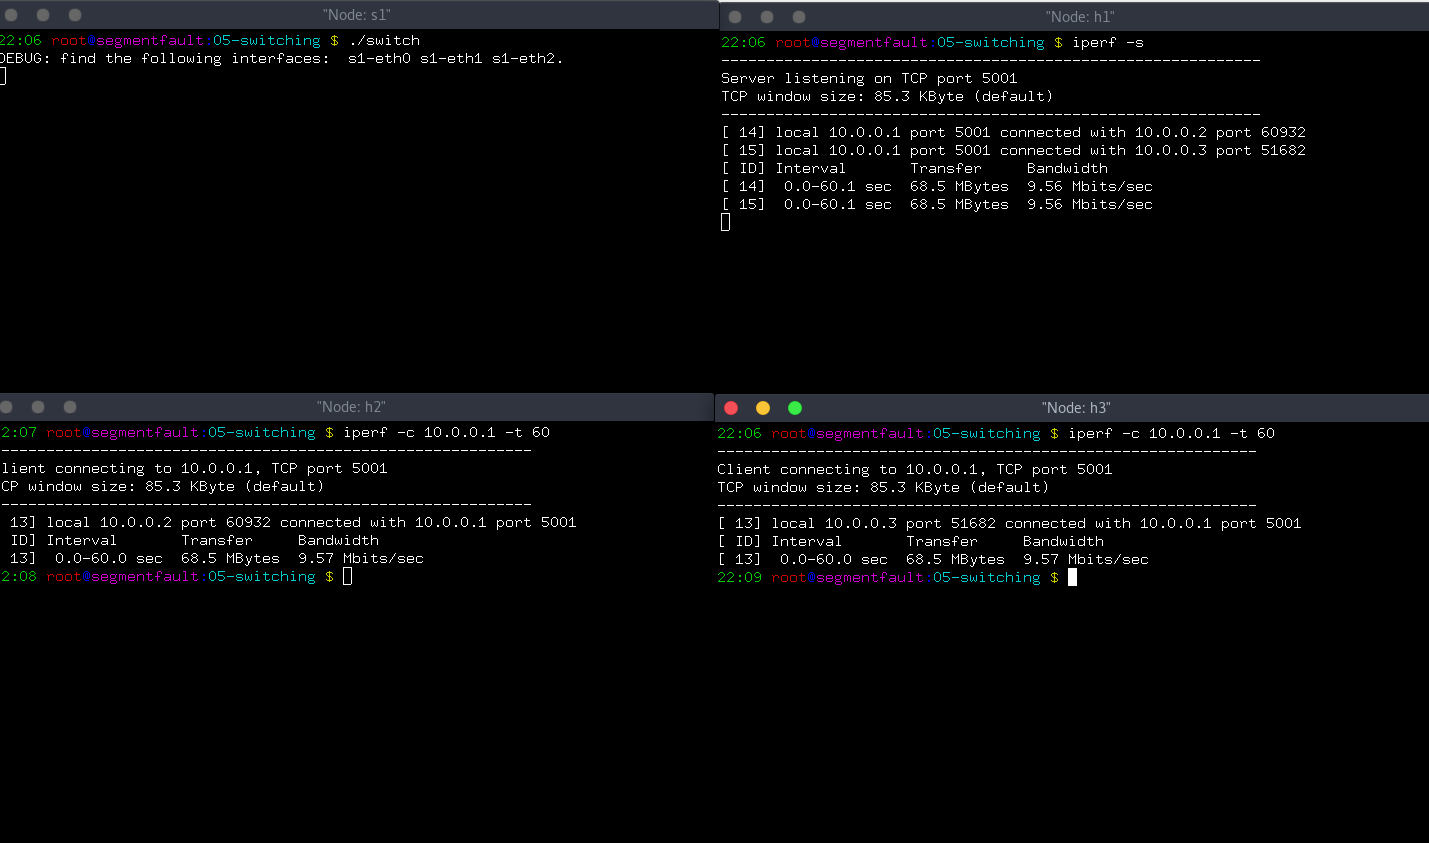
\includegraphics[scale=0.3]{1.png}
  \caption{使用$iperf$进行性能测量}
\end{figure}

和广播性能对比:
\begin{itemize}
  \item $h1\ server, h2/h3 clients$:同时向$h1$发送包,测得$h1$的带宽为$17.96MB/s$,链路利用率为$89.8\%$,$h2$带宽均为$9.16MB/s$,利用率为$91.6\%$,$h3$带宽为$8.98MB/s$,链路利用率为$89.8\%$;
  \item $h1\ client, h2/h3 severs$:$h1$带宽分别为$9.41MB/s$和$9.43MB/s$,$h2,h3$带宽均为$9.37MB/s$。
\end{itemize}

通过对比可知,转发机的链路利用率比广播网络要高。

		\section*{{\CJKfamily{zhhei}结果分析}}
		在交换机中,每一个包都有目的地址,因此,可以实现多个数据包的同时传输,而在广播网络中,同一时刻只能有一个数据包进行传输,还可能发生碰撞,因此,交换机的性能要比广播网络的性能好。
			%\hline
			%  \end{tabular}
			%\end{center}
			\end{document}


